\chapter{Forces and Newtons Laws} \index{Newton's Laws of Motion}
\section{Forces}
\gls{force} is a vector quantity that measures how hard a push or a pull on an object is.  Though all forces we encounter in everyday life can be explained in terms of the four \gls{fundamentalforces}, these forces manifest themselves in different ways.  In fact, with the exception of gravity, almost all forces humans deal with are electromagnetic.  

 \section{Free Body Diagrams}
\index{Free Body Diagram}
A \gls{freebodydiagram} is a diagram that includes all external forces acting on an object or system.  In general, free body diagrams should follow the following rules:
\begin{itemize}
	\item Draw a coordinate system, which shows what direction is +x and +y.
	\item Objects should be represented by a dot, a box, or a sketch of the object.  Systems can be represented by multiple dots, boxes, or sketches.  
	\item Unless otherwise stated, forces act on the center of mass.
	\item Forces are represented as arrows.  Arrows should start at the center of mass (or other point they act on) and point away from the object.  
	\item The length of force arrows should be proportional to the strength of the force.
	\item All forces should be labeled.
	\item No arrows other than forces should appear on the diagram.  (Don't include accleration, displacements, velocities, etc.) 	
\end{itemize}
\newpage

\begin{mdframed}[backgroundcolor=blue!10!white]
	\begin{center}
		
		
		\textbf{Example \thesection.1}	
	\end{center}
	
	\textbf{Problem: } A book is at rest on top of a table.  Draw the free-body diagram of the book on the table.
	\vspace{0.1in}
	
	\textbf{Solution:} 
	The diagram should look as follows:
	\begin{center}
		
		
		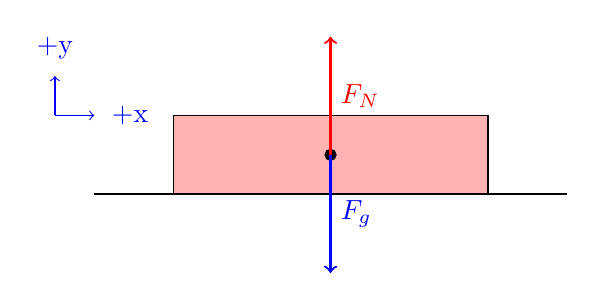
\begin{tikzpicture}
			
			% Draw the book
			\draw[fill=red!30] (0,0) rectangle (4,1); % The book as a rectangle
			%	\node at (2,0.5) {}; % Label for the book
			
			% Draw the table (optional)
			\draw[thick] (-1,0) -- (5,-0); % Table surface
			
			% Center of Mass (dot in the middle)
			\filldraw[black] (2,0.5) circle (2pt); % Dot for the center of mass
			%		\node at (2.5,0.8) {};
			
			% Draw the forces acting on the book
			% Normal force (upward)
			\draw[->, thick, red] (2,0.5) -- (2,2) node[midway, right] {$F_N$};
			
			% Weight (downward)
			\draw[->, thick, blue] (2,0.5) -- (2,-1) node[midway, right] {$F_g$};
			
			% Add labels for the diagram
			%	\node at (2,-2) {Free Body Diagram of a book on a table};
			%Draw the coordinate system
			\draw[->,blue] (-1.5,1) -- (-1.5,1.5);
			\node at (-1.5,1.6) [above,blue] {+y};
			
			\draw[->,blue] (-1.5,1) -- (-1,1);
			\node at (-0.9,1) [right,blue] {+x};
			
		\end{tikzpicture}
	\end{center}
	
	In this diagram, the normal force and the gravitational force are balanced.  Thus, the object remains at rest, according to Newton's 1st Law.  
	
\end{mdframed}	



\begin{mdframed}[backgroundcolor=blue!10!white]
	\begin{center}

		
		\textbf{Example \thesection.2}	
	\end{center}
	
	\textbf{Problem: } As a person walks through an airport, she pulls a suitcase at a constant speed using a strap at a 25 degree angle above horizontal.  Friction is significant.  Draw a free body diagram of the situation.
	\vspace{0.1in}
	
	\textbf{Solution:} 
	The diagram should look as follows:
	
	\begin{center}
		
		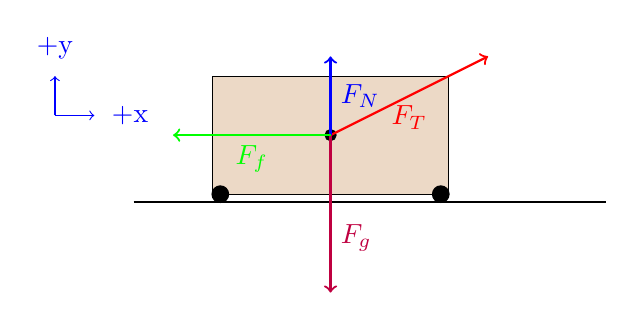
\begin{tikzpicture}
			
			% Draw the suitcase
			\draw[fill=brown!30] (0,0) rectangle (3,1.5); % Suitcase as a rectangle
			%	\node at (1.5,0.75) {Suitcase}; % Label for suitcase
			\draw[fill=black] (0.1,0) circle (3 pt); % wheel 1
			\draw[fill=black] (2.9,0) circle (3 pt); % wheel 2
			
			
			% Draw the ground (optional)
			\draw[thick] (-1,-0.1) -- (5,-0.1); % Ground line
			
			% Center of mass (dot in the middle)
			\filldraw[black] (1.5,0.75) circle (2pt); % Dot for center of mass
			
			% Draw the forces acting on the suitcase
			% Tension force (pulling force at 25-degree angle)
			\draw[->, thick, red] (1.5,0.75) -- ++(2,1) node[midway, below] {$F_T$};
			%\node at (1.6,0.75) [right,red] {$25^\circ$}; % Angle of the tension force
			
			% Normal force (upward)
			\draw[->, thick, blue] (1.5,0.75) -- ++(0,1) node[midway, right] {$F_N$};
			
			% Weight force (downward)
			\draw[->, thick, purple] (1.5,0.75) -- (1.5,-1.25) node[midway, below right] {$F_g$};
			
			% Friction force (leftward)
			\draw[->, thick, green] (1.5,0.75) -- (-0.5,0.75) node[midway, below] {$F_f$};
			
			% Add labels for the diagram
			%	\node at (1.5,-1.8) {Free Body Diagram of a suitcase being pulled at a 25-degree angle};
			
			
			%Draw the coordinate system
			\draw[->,blue] (-2,1) -- (-2,1.5);
			\node at (-2,1.6) [above,blue] {+y};
			
			\draw[->,blue] (-2,1) -- (-1.5,1);
			\node at (-1.4,1) [right,blue] {+x};
		\end{tikzpicture}
		
		
		
	\end{center}
	
	In this diagram, the sum of the forces that act in the x-direction (friction, and the x-component of tension) must equal zero to ensure the suitcase maintains a constant horizontal speed.  In addition, the forces that act in the y-direction (Gravity, Normal Force, and the Y-component of tension) must sum to equal zero as well so that the suitcase does not accelerate vertically.  
	
\end{mdframed}	


\newpage
	\section{Newton's First Law} \index{Newton's First Law} \index{Law of Inertia}
	\begin{tabular}{p{.75in} p{4.5in} p{.75in}}
		 & \textit{Corpus omne perseverare in statu suo quiescendi vel movendi uniformiter in directum, nisi quatenus a viribus impressis cogitur statum illum mutare.} &  \\
		  & & \\
		 & \textit{Every body continues in its state of being at rest or moving uniformly in a direction, except insofar as it is compelled to change its state by means of an imparted force. } & \\
		 & & \\

		&  -- Newton, Isaac.  \textit{Philosophiae Naturalis Principia Mathematica}.  tr. J. Williamson & \\
		& & \\
	\end{tabular}

	

	
  You may have heard Sir Isaac Newton's first law of physics stated in different ways than the above.  Often in grade school, students are taught a phrase beginning with ``objects in motion...''.  	Sometimes this law is called the ``Law of Inertia''.   This is a very basic understanding of the complexity of this law.  In fact, all non-accelerating systems are governed by this law.  As long as the vector sum of the forces upon an object is zero, the object will continue in a state of uniform motion (remaining at rest is a type of uniform motion) until something causes the equilibrium of the system to be lost.  
	Likewise, if an object is known to have an acceleration of zero, we can state that the vector sum of the forces is equal to zero.  We can use this law to characterize non-accelerating systems:
	
				\begin{mdframed}[backgroundcolor=orange!20!white]
		\begin{equation}
			\Sigma \vec{F} = 0  
			\label{eqn:newtonsfirst}
		\end{equation}
	\end{mdframed}

\newpage

	
	\section{Newton's Second Law}
	\index{Newton's Second Law}
		\begin{tabular}{p{.75in} p{4.5in} p{.75in}}
		& \textit{Mutationem motus proportionalem esse vi motrici impressae, et fieri secundum lineam rectam qua vis illa imprimitur.} &  \\
		& & \\
		& \textit{The change in motion is proportional to the amount of force of motion imparted, and according to the straight line made by the force impressed. } & \\ 
		& & \\
		 & {-Newton, Isaac.  \textit{Philosophiae Naturalis Principia Mathematica}.  tr. J. Williamson} & \\		
		 	& & \\
	\end{tabular}

Newton's Second Law describes objects and systems that have a constant acceleration.  The vector sum of the forces on an object is equal to the object's mass times its acceleration:

				\begin{mdframed}[backgroundcolor=orange!20!white]
	\begin{equation}
		\Sigma \vec{F} = m \vec{a}  
		\label{eqn:newtonssecond}
	\end{equation}
\end{mdframed}
	
	It should be noted that forces are vectors.  Thus, when forces are combined, their directions should be taken into account.  The direction of the net force is always in the same direction as the acceleration of the object. 
	
	It should also be noted that if all the forces on an object cancel, the acceleration of the object will be zero - which means that the first law is just a special case of the second law when $\Sigma F = 0 N$.
	
	Often, if the forces on an object of known mass can be determined, the acceleration of the object can also be determined.  The acceleration found using Newton's second law can then be used in kinematic equations to determine other important quantities. 
	
	\subsection{Mass and Weight}
	In everyday language, we often use the words \gls{mass} and \gls{weight} interchangeably — but in physics, they refer to two very different things.
	
	\textbf{Mass} is a measure of how much matter an object contains. It is an intrinsic property of an object and does not change based on location. Whether you're on Earth, the Moon, or floating in space, your mass remains the same. Mass is measured in kilograms (kg) in the SI system.
	
	\textbf{Weight}, on the other hand, is the force of gravity acting on an object with mass. It depends not only on the object’s mass but also on the strength of the local gravitational field. Weight is a force and is measured in newtons (N).
	
	The formula to calculate an object's weight is:
	\[
	W = F_g = mg
	\]
	where \( m \) is the mass of the object in kilograms and \( g \) is the local gravitational acceleration.  It should be noted that on earth:
	
			\begin{mdframed}[backgroundcolor=green!20!white]
		\begin{equation*}
			g  = \SI{9.81}{m/s^2}
			\label{constant:gearth}
		\end{equation*}
	\end{mdframed}	
	
	For example, a person with a mass of \( 70 \, \text{kg} \) has a weight of:
	\[
	W = (70 \, \text{kg})(9.81 \, \text{m/s}^2) = 686.7 \, \text{N}
	\]
	
	This distinction is important: \textbf{mass stays the same everywhere}, but \textbf{weight depends on gravity}.
	
	
	 \subsection{Normal Force}
	 \index{Normal Force}
	 \gls{normalforce}s are contact forces exerted by a surface that supports the weight of an object resting on it. It acts \textbf{perpendicular} (or "normal") to the surface.
	 
	 The normal force prevents objects from falling through solid surfaces. When you stand on the floor, your weight pulls you down due to gravity, and the floor pushes back up on you with a force of equal magnitude — this is the normal force. It’s a reactive force: it exists only when there is contact, and its value adjusts to balance other vertical forces.
	 
	 In many situations, especially when a surface is horizontal and there’s no vertical acceleration, the normal force exactly balances the object’s weight:
	 \[
	 F_N = mg
	 \]
	 
	 However, if there is vertical acceleration — such as in an elevator or on a roller coaster — the normal force may be larger or smaller than \( mg \), depending on the direction of acceleration.
	 
	 On inclined planes, the normal force does not equal the object's weight. Instead, it balances only the component of weight \textbf{perpendicular} to the surface:
	 \[
	 F_N = mg \cos\theta
	 \]
	 where \( \theta \) is the angle of the incline.
	 
	 Understanding the normal force is key to solving problems involving contact forces, friction, and apparent weight.
	 
	
	\section{Newton's Third Law}
	\index{Newton's Third Law}
		\begin{tabular}{p{.75in} p{4.5in} p{.75in}}
		&  &  \\
		& & \\
		& \textit{Actioni contrariam semper et aequalem esse reactionem: sive corporum duorum actiones in se mutuo semper esse aequales et in partes contrarias dirigi. } & \\
		& & \\
		& \textit{For an action there is always an equal and opposite reaction: or the two bodies on each other are always equal and in opposite directions. } & \\
		& & \\
		 & {-Newton, Isaac.  \textit{Philosophiae Naturalis Principia Mathematica}.  tr. J. Williamson} & \\
		
	\end{tabular}
	
	This law is often stated "For every action, there is an equal, opposite reaction."  Perhaps a better understanding of this law would directly deal with forces: "For every force, there is an equal, opposite reaction force."  This means that whenever object A puts a force on object B, object B puts a force on object A that is the same strength and in the opposite direction.  Some examples might include:
	\begin{itemize}
		\item You push on the wall to the left.  The wall pushes on you to the right.
		\item One magnet pulls a piece of metal to the left.  The metal pulls the magnet to the right.
		\item When swimming, you push water backward.  The water pushes you forward.  
		\item The Earth's gravity pulls downward on you.  You pull the earth upward with the same amount of force.
		\item A jet engine pushes air backward.  The air pushes the engine (and the plane it's connected to) forward.
	\end{itemize}
	There are countless examples of Newton's Third Law pairs - in fact, every force has a corresponding reaction force.  It is important to remember, however, that while the forces must be equal, the resulting accelerations will not be unless the mass of the objects is equal.  
	
	\newpage
	
	\section{Applications of Newton's Laws}
		\subsection{Friction}
		\index{Friction}
		\gls{friction} occurs whenever two surfaces are in contact, and it is a force that has two effects.  
		\begin{itemize}
			\item Friction always opposes the motion of an object, or even the tendency to move.
			\item Friction dissipates energy into heat.
		\end{itemize}
		
		\index{Friction, static} \index{Friction, kinetic}
		There are two types of friction that one should know about: \textbf{static friction} and \textbf{kinetic friction}.  Static friction is present when two surfaces are in contact, but not sliding.  Kinetic friction is occurs when two surfaces are in contact and sliding past each other.  One should note that when an object is rolling, there is static friction between the outer edge of the wheel and the surface it is rolling on, whereas static or kinetic friction may be present where the wheel is connected to the axle, depending on the type of joint that is used.  
		
		\index{Coefficient of Friction}
		The \textbf{coefficient of static friction}  and the \textbf{coefficient of kinetic friction}, symbolized by $\mu_s$ and $\mu_k$ respectively, measure how hard it is to slide two surfaces past each other.  A surface that is very slippery will have low coefficients of friction, whereas surfaces that grip each other well will very high coefficients of friction. A perfectly frictionless surface would have a coefficient of friction of 0.  Some examples of coefficients of friction can be found in \color{red} insert reference here\color{black}.  One should also note that the coefficients of friction are unitless.  
		
		To calculate the force of static friction, the following formula is used:
		\index{Static Friction}
		\index{Friction, static}
		\begin{mdframed}[backgroundcolor=orange!20!white]
			\begin{equation}
				|F_f| \leq \mu_s |F_N|  
				\label{eqn:frictionstatic}
			\end{equation}
		\end{mdframed}
	
	The force of kinetic friction can be calculated by using this formula:
			\index{Friction, kinetic}
			\index{Kinetic Friction}
			\begin{mdframed}[backgroundcolor=orange!20!white]
		\begin{equation}
			|F_f| = \mu_k |F_N|  
			\label{eqn:frictionkinetic}
		\end{equation}
	\end{mdframed}


		
		\begin{mdframed}[backgroundcolor=blue!10!white]
			\begin{center}
				
				
				\textbf{Example \thesection.1}	
			\end{center}
			
			\textbf{Problem: } In the game of curling, a stone of mass 19.1 kg is pushed across the ice with an initial speed of 4 m/s.  The coefficient of kinetic friction is 0.045.  How far does the rock slide until it comes to a stop?
			\vspace{0.1in}
			
			\textbf{Solution:} 
			First, draw a free body diagram:
			
			\begin{center}
				
				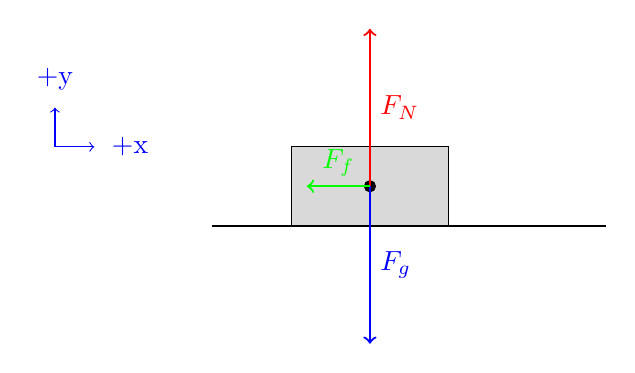
\begin{tikzpicture}
				
				% Draw the rock
				\draw[fill=gray!30] (0,0) rectangle (2,1); % Rock as a rectangle
			%	\node at (1,0.5) {Rock}; % Label for rock
				
				% Draw the ground (optional)
				\draw[thick] (-1,-0) -- (4,-0); % Ground line (ice)
				
				% Center of mass (dot in the middle)
				\filldraw[black] (1,0.5) circle (2pt); % Dot for center of mass
				
				% Draw the forces acting on the rock
				% Gravity (downward)
				\draw[->, thick, blue] (1,0.5) -- (1,-1.5) node[midway, right] {$F_g$};
				
				% Normal force (upward)
				\draw[->, thick, red] (1,0.5) -- (1,2.5) node[midway, right] {$F_N$};
				
				% Friction force (leftward)
				\draw[->, thick, green] (1,0.5) -- (0.2,0.5) node[midway, above] {$F_f$};
				
				% Add labels for the diagram
%				\node at (1,-2) {Free Body Diagram of a rock sliding on ice};
				
					
				%Draw the coordinate system
				\draw[->,blue] (-3,1) -- (-3,1.5);
				\node at (-3,1.6) [above,blue] {+y};
				
				\draw[->,blue] (-3,1) -- (-2.5,1);
				\node at (-2.4,1) [right,blue] {+x};
				
				\end{tikzpicture}
				
				
			\end{center}
			Since the mass of the rock is known, we can find the force of gravity:
			
			\begin{equation*}
			\vec{F}_g = m g = (\SI{19.1}{kg})(\SI{-9.81}{m/s^2}) \approx \SI{-187.371}{N}
			\end{equation*}
		
			Since the rock is not accelerating in the y-direction, the normal force must be equal in magnitude to gravity, and in the opposite direction.
			
			\begin{equation*}
			\vec{F}_N \approx \SI{187.371}{N}
			\end{equation*}
			
			The normal force is now known, so we can find the force of friction on the rock:
			\begin{equation*}
			|F_f| = \mu_k |F_N|   = (0.045)( \SI{187.371}{N}) \approx \SI{8.432}{N} 
			\end{equation*}
			Since the force of friction is to the left, we assign a negative value to it:
				\begin{equation*}
			F_f \approx \SI{-8.432}{N} 
			\end{equation*}
			Newton's 2nd Law allows us to find the acceleration of the rock, since the only unbalanced force is friction.
			\begin{equation*}
			\Sigma \vec{F} = m \vec{a} \longrightarrow \vec{a} = \frac{\Sigma \vec{F}}{m} = \frac{\vec{F}_f}{m} =  \frac{\SI{-8.432}{N}}{\SI{19.1}{kg}} \approx \SI{-0.442}{m/s^2}
			\end{equation*}
			
			Using kinematic equations allows us to find the distance:
			\begin{equation*}
			\vec{v}^2 = \vec{v}_0^2 + 2 \vec{a}(\vec{x}-\vec{x}_0) \longrightarrow  (\vec{x}-\vec{x}_0) = \frac{\vec{v}^2 - \vec{v}_0^2}{2 \vec{a}} = \frac{(\SI{0}{m/s})^2 - (\SI{4}{m/s})^2}{2 (\SI{-0.442}{m/s^2})} \approx \SI{18.120}{m}
			\end{equation*}
			
			
		\end{mdframed}	
	
	
		\newpage
		
	\begin{mdframed}[backgroundcolor=blue!10!white]
		\begin{center}
		
			
			\textbf{Example \thesection.2}	
		\end{center}
		
		\textbf{Problem: } A 2-kg mass is placed on top of a table.  It is connected to a string that runs through a pulley at the edge of the table, which subsequently is connected to a mass that hangs off the table, as shown in the diagram. 
		
		\begin{center}
			
		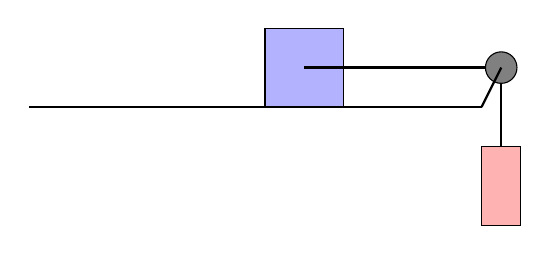
\begin{tikzpicture}
			
			% Draw the table
			\draw[thick] (-2,-0.5) -- (3.75,-0.5); % Table surface
			
			% Draw the 2kg mass on the table
			\draw[fill=blue!30] (1,-0.5) rectangle (2,0.5); % Block on table
			%\node at (1.5,0) {2 kg}; % Label for block
			
			% Draw the string and pulley
			\draw[thick] (1.5,0) -- (4,0); % x part of the string
			\draw[thick] (4,0) -- (4,-1); % y part of the string
			\draw[fill=gray] (4,0) circle (0.2); % Pulley
			\draw[thick] (3.75,-.5) -- (4,0); % pulley support
			
			% Draw the hanging mass (0.423 kg)
			\draw[fill=red!30] (3.75,-1) -- (3.75,-2) -- (4.25,-2) -- (4.25,-1) -- cycle; % Hanging mass
			%\node at (4.25,1.5) {0.423 kg}; % Label for hanging mass
			
		
			
		\end{tikzpicture}
	\end{center}	
		
		
		  A student finds that the largest mass that can be held by the string without the mass on the table moving is 0.423 kg.  What is the coefficient of static friction between the table and the 2 kg mass?
		\vspace{0.1in}
		
		\textbf{Solution:} 
		First, draw a free body diagram:
		
		\begin{center}
			
		
				
				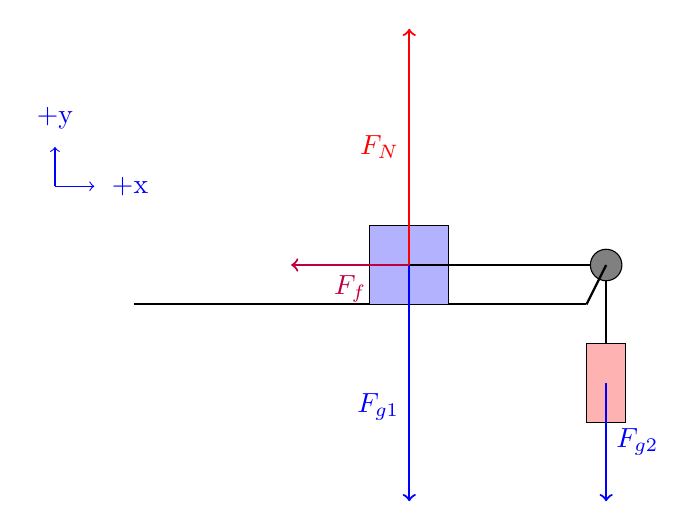
\begin{tikzpicture}
					
					% Draw the table
					\draw[thick] (-2,-0.5) -- (3.75,-0.5); % Table surface
					
					% Draw the 2kg mass on the table
					\draw[fill=blue!30] (1,-0.5) rectangle (2,0.5); % Block on table
					%\node at (1.5,0) {2 kg}; % Label for block
					
					% Draw the string and pulley
					\draw[thick] (1.5,0) -- (4,0); % x part of the string
					\draw[thick] (4,0) -- (4,-1); % y part of the string
					\draw[fill=gray] (4,0) circle (0.2); % Pulley
						\draw[thick] (3.75,-.5) -- (4,0); % pulley support
					
					% Draw the hanging mass (0.423 kg)
					\draw[fill=red!30] (3.75,-1) -- (3.75,-2) -- (4.25,-2) -- (4.25,-1) -- cycle; % Hanging mass
					%\node at (4.25,1.5) {0.423 kg}; % Label for hanging mass
					
					% Forces on the 2kg mass
					\draw[->, thick, blue] (1.5,0) -- (1.5,-3) node[midway, below left] {$F_{g1}$}; % Weight of 2kg mass
					\draw[->, thick, red] (1.5,0) -- (1.5,3) node[midway, left] {$F_N$}; % Normal force
				%	\draw[->, thick, green] (2.1,0) -- (3,0) node[midway, below] {$F_T$}; % Tension in string
					
					% Forces on the hanging mass (0.423kg)
					\draw[->, thick, blue] (4,-1.5) -- (4,-3) node[midway, right] {$F_{g2}$}; % Weight of 0.423kg mass
					
					% Friction force on the 2kg block
					\draw[->, thick, purple] (1.5,0) -- (-0,0) node[midway, below] {$F_f$}; % Friction force
					
					% Labels and notes
				%	\node at (2,-2) {Free Body Diagram of the system};
%					\node at (3.8,0.2) {Pulley (ideal, frictionless)};
					
						%Draw the coordinate system
					\draw[->,blue] (-3,1) -- (-3,1.5);
					\node at (-3,1.6) [above,blue] {+y};
					
					\draw[->,blue] (-3,1) -- (-2.5,1);
					\node at (-2.4,1) [right,blue] {+x};
					
				\end{tikzpicture}
				
			
				
		
			
			
		\end{center}
	One should note that tension in the string is not shown on the free body diagram, because tension in the string is a force that is internal to the system.
	
	We can find the force of gravity on the 2 kg mass:
		
		\begin{equation*}
			\vec{F}_{g1} = m_1 g = (\SI{2}{kg})(\SI{-9.81}{m/s^2}) \approx \SI{-19.62}{N}
		\end{equation*}
		
		The 2 kg mass does not accelerate vertically, so we know that the normal force must be equal to the force of gravity, $F_{g1}$:
		
		\begin{equation*}
			\vec{F}_N \approx \SI{19.62}{N}
		\end{equation*}
		
		We can also find the force of gravity on the hanging mass.  
			\begin{equation*}
			\vec{F}_{g2} = m_2 g = (\SI{0.423}{kg})(\SI{9.81}{m/s^2}) \approx \SI{4.150}{N}
		\end{equation*}
		You can think of the x-axis of the coordinate system as wrapped around the pulley in the same way the string goes around it, so this force is in the +x direction.  This means that static friction is the same magnitude, but in the -x direction.
		
			\begin{equation*}
			\vec{F}_f \approx \SI{-4.150}{N}
		\end{equation*}
		 
		 Now, we can use equation \ref{eqn:frictionstatic} to calculate the coefficient of friction.  
		 
		 	\begin{equation*}
		 	|F_f| \leq \mu_s |F_N|  
		 \end{equation*}
		 
		 Because this is the greatest amount of mass that can be attached without causing the 2 kg mass to slide, the force of friction must be at its greatest amount, so:
		 
		 \begin{equation*}
		 	|F_f| = \mu_s |F_N|  \longrightarrow \mu_s = \frac{|F_f|}{|F_N|} = \frac{|\SI{-4.150}{N}|}{|\SI{19.62}{N}|} \approx 0.212
		 \end{equation*}
		 
		
	\end{mdframed}	
	
	
	\newpage
		
		\subsection{Inclined Planes}
		\index{Inclined Plane} The normal force that a surface exerts on an object is always perpendicular to the surface.  Thus, when an object is placed on an inclined plane, the normal force exerted on the object will not be vertical.  Similarly, any frictional forces will be parallel to the inclined plane, and the motion of the object will be along the plane as well.  Thus, it is easier to deal with inclined planes by creating a coordinate system that is rotated to align with the inclined plane, as seen in the figure below:
		
		
		
		
		
		\newcommand{\angler}{30}
		\begin{figure}[H]
			\centering
		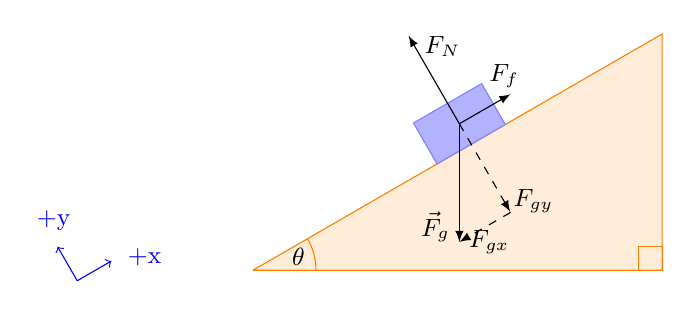
\begin{tikzpicture} [font = \small]
			
			% triangle:
			\draw [draw = orange, fill = orange!15] (0,0) coordinate (O) -- (\angler:6)
			coordinate [pos=.45] (M) |- coordinate (B) (O);
			
			% angles:
			\draw [draw = orange] (O) ++(.8,0) arc (0:\angler:0.8) 
			node [pos=.4, left] {$\theta$};
			\draw [draw = orange] (B) rectangle ++(-0.3,0.3);
			
			\begin{scope} [-latex,rotate=\angler]
				
				% Object (rectangle)
				\draw [fill = blue!30,
				draw = blue!50] (M) rectangle ++ (1,.6);
				
				% Weight Force and its projections
				\draw [dashed] (M) ++ (.5,.3) coordinate (MM) -- ++ (0,-1.29)
				node [very near end, right] {$F_{gy}$};
				
				\draw [dashed] (3.2,-1) -- ++ (-0.75,0) 
				node [right] {$F_{gx}$};
				
				\draw (MM) -- ++ (-\angler-90:1.5)
				node [very near end,left ] {$\vec{F}_g$};
				
				% Normal Force
				\draw (MM) -- ++ (0,1.29)
				node [very near end, right] {$F_N$};
				
				% Frictional Force
				\draw (MM) -- ++ (0.75,0)
				node [very near end, above] {$F_f$};
				
						%Draw the coordinate system
				\draw[->,blue] (-2,1) -- (-2,1.5);
				\node at (-2,1.6) [above,blue] {+y};
				
				\draw[->,blue] (-2,1) -- (-1.5,1);
				\node at (-1.4,1) [right,blue] {+x};
				
				
			\end{scope}
			
		\end{tikzpicture} 
		\caption{An inclined plane}
				\end{figure}
		In this case, we have chosen to make the positive x direction up the ramp, and the positive y direction upward and to the left, perpendicular to the ramp.  This means that the normal force is in the postive y direction, and the frictional force is in the positive x direction.  The only force that does not align to the coordinate system is gravity.  However, it is easy to decompose gravity into two forces, one in the x-direction and one in the y-direction, as shown by the dashed arrows in the diagram. 
		A little geometry proves that $F_{gx} = F_g \sin (\theta) $ and $F_{gx} = F_g \cos (\theta)$.  We can then assign positives and negatives based on the coordinate system we have chosen.  
		
		
		
		
		\subsection{Elevators}
		\index{Elevator}
		\index{Apparent Weight}
		Have you ever felt heavier as an elevator begins to rise, or lighter as it starts to descend? That strange sensation isn’t just in your head — it’s a measurable difference in what’s called your \gls{apparentweight}. It’s the force your body feels as it presses against the floor, or what a bathroom scale would read during the motion.
		
		In physics, your \textbf{actual weight} is the gravitational force acting on you, given by \( W = mg \). This doesn't change unless your mass or the local gravitational field changes. But your \textbf{apparent weight} depends on how the floor pushes back on you — in other words, the \textbf{normal force}. In situations like elevators, where acceleration is involved, this normal force may increase or decrease, making you feel heavier or lighter even though your true weight remains the same.
		
		
		
		
		\subsection{Pulleys and Atwood Machines}
		\index{Atwood Machine}
		

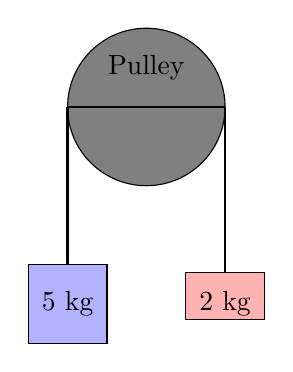
\begin{tikzpicture}
	
	% Draw the pulley
	\draw[fill=gray] (0,2) circle (1); % Pulley as a circle
	\node at (0,2.5) {Pulley};
	
	% Draw the string going over the pulley
	\draw[thick] (-1,2) -- (1,2); % Horizontal string
	\draw[thick] (-1,2) -- (-1,0); % Left vertical string segment
	\draw[thick] (1,2) -- (1,-0.1); % Right vertical string segment
	
	% Draw the 5 kg mass on the left side
	\draw[fill=blue!30] (-1.5,0) rectangle (-.5,-1); % Mass box
	\node at (-1,-.5) {5 kg}; % Label for the 5 kg mass
	
	% Draw the 2 kg mass on the right side
	\draw[fill=red!30] (0.5,-0.1) rectangle (1.5,-.7); % Mass box
	\node at (1,-.5) {2 kg}; % Label for the 2 kg mass
	
	% Add arrows to represent forces (optional)
	% Gravity on 5 kg mass
	%\draw[->, thick, blue] (-1.5,-0.5) -- (-1.5,-1.5) node[midway, left] {};
	% Gravity on 2 kg mass
	%\draw[->, thick, red] (1.5,-0.5) -- (1.5,-1.5) node[midway, right] {};
	
\end{tikzpicture}
	


